\section{Boundary Conditions}
In order to understand how to implement boundary conditions, we shall 
first describe the general principles behind working with boundary conditions.
Then, we will provide simple examples in the tutorial directory that can be 
adapted to other applications.

\subsection{General Principles}
The basic idea is that every grid has knowledge of the
boundary condition type at the low and high side edge in each direction.
Common boundary condition types are {\tt INFLOW}, {\tt OUTFLOW}, {\tt SLIP\_WALL},
{\tt NO\_SLIP\_WALL}, and {\tt PERIODIC}.
There is also an {\tt INTERIOR} boundary condition type, which 
will be explained below.  There is typically an integer mapping, e.g., {\tt INFLOW}=1,
{\tt OUTFLOW=2}, etc.  Consider grid 1 in Figure \ref{fig:bc_example1}.  The
low-x boundary condition is {\tt INFLOW}, and the high-y boundary condition is
{\tt NO\_SLIP\_WALL}.  The high-x and low-y boundary conditions are {\tt INTERIOR}, which
means that the ghost cells share the same physical space as cells in the valid region of 
another grid.  Note that for grids 6, 7, 10, and 11, the boundary condition type for
every side is {\tt INTERIOR}.
%%%%%%%%%%%%%%%%%%%%%%%%%%%%%%%%%%%%%
\begin{figure}[tb]
\centering
\includegraphics[width=4in]{./AdvancedTopics/bc_example1}
\caption{\label{fig:bc_example1}Two-dimensional example with 16 - 4$^2$grids with
{\tt INFLOW}, {\tt OUTFLOW}, and {\tt NO\_SLIP\_WALL} boundary conditions.
The numbers refer to the grid number.}
\end{figure}
%%%%%%%%%%%%%%%%%%%%%%%%%%%%%%%%%%%%%

Figure \ref{fig:bc_example2} demonstrates a problem with periodicity.  In this case,
the low-x boundary condition for grid 1 is {\tt PERIODIC}.  Note there are some
similarities between {\tt PERIODIC} and {\tt INTERIOR} boundary conditions when
it comes to filling ghost cells.  In fact, one can think of {\tt PERIODIC} as just
a special type of {\tt INTERIOR} boundary condition.
In both of these cases, when filling ghost cells,
data from the valid region of another grid is copied into ghost cells of the neighboring 
grid.  For the other boundary conditions types, the user can write custom boundary 
conditions routines to fill ghost cells, which can involve setting ghost cell values 
directly, or extrapolating values from interior points using some stencil.
%%%%%%%%%%%%%%%%%%%%%%%%%%%%%%%%%%%%%
\begin{figure}[tb]
\centering
\includegraphics[width=4in]{./AdvancedTopics/bc_example2}
\caption{\label{fig:bc_example2}Two-dimensional example with 16 - 4$^2$grids with
{\tt PERIODIC} and {\tt NO\_SLIP\_WALL} boundary conditions.
The numbers refer to the grid number.}
\end{figure}
%%%%%%%%%%%%%%%%%%%%%%%%%%%%%%%%%%%%%

Now, consider an example with refined grids.  Figure \ref{fig:bc_example3}
contains three grids at the next level of refinement.  In this case, for grid 1,
all of the boundary condition types are {\tt INTERIOR}, even though the neighboring
valid region data is at a coarser level of refinement.  For grid 2, the low-y
boundary condition is {\tt NO\_SLIP\_WALL}, and the low-x, high-x, and hi-y
boundary condition types are {\tt INTERIOR}.
%%%%%%%%%%%%%%%%%%%%%%%%%%%%%%%%%%%%%
\begin{figure}[tb]
\centering
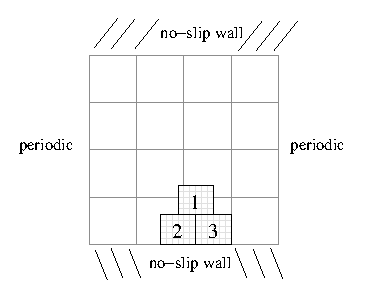
\includegraphics[width=4in]{./AdvancedTopics/bc_example3}
\caption{\label{fig:bc_example3}Two-dimensional example with 3 grids at a finer
resolution than the base grid.}
\end{figure}
%%%%%%%%%%%%%%%%%%%%%%%%%%%%%%%%%%%%%

\subsection{Fortran90 Tutorial}

\section{Nodal Data}

\section{Checkpoints and Restarting}

\section{Linear Solvers}

\section{Adaptive Mesh Refinement}

\section{OpenMP and Threads}
